%%%%%%%%%%%%%%%%%%%%%%%%%%%%%%%%%%%%%%%%%%%%%%%%%%%%%%%%%%%%%%%%%%%%%%%%
% Beamer Presentation - LaTeX - Template Version 1.0 (10/11/12)
% This template has been downloaded from: http://www.LaTeXTemplates.com
% License: % CC BY-NC-SA 3.0 (http://creativecommons.org/)
% Modified by Rahmat M. Samik-Ibrahim
% REV224 Mon Apr  6 00:35:14 WIB 2020
% REV156 Mon Aug 27 15:03:00 WIB 2018
% STARTX Mon Aug 13 20:51:13 WIB 2018
%%%%%%%%%%%%%%%%%%%%%%%%%%%%%%%%%%%%%%%%%%%%%%%%%%%%%%%%%%%%%%%%%%%%%%%%%

% PACKAGES AND THEMES ZCZC
\documentclass[xcolor=table, notheorems, hyperref={pdfpagelabels=false}]{beamer}
%%%%%%%%%%%%%%%%%%%%%%%%%%%%%%%%%%%%%%%%%%%%%%%%%%%%%%%%%%%%%%%%%%%%%%%%
% Beamer Presentation - LaTeX - Template Version 1.0 (10/11/12)
% This template has been downloaded from: http://www.LaTeXTemplates.com
% License: % CC BY-NC-SA 3.0 (http://creativecommons.org/)
% Modified by Rahmat M. Samik-Ibrahim
% REV316 Wed 14 Jul 2021 13:42:41 WIB
% REV217 Tue Feb  4 15:10:30 WIB 2020
% REV198 Wed Mar 13 16:39:02 WIB 2019
% REV006 Mon Jan 22 19:10:41 WIB 2018
% REV005 Mon Oct  2 14:45:07 WIB 2017
% START  Thu Aug 25 14:15:19 WIB 2016
%%%%%%%%%%%%%%%%%%%%%%%%%%%%%%%%%%%%%%%%%%%%%%%%%%%%%%%%%%%%%%%%%%%%%%%%%

%% ZCZC NNNN
\newtheorem{example}{Example}

%%%%%%%%%%%%%%%%%%%%%%%%%%%%%%%%%%%%%%%%%%%%%%%%%%%%%%%%%%%%%%%%%%%%%%%%%

\let\Tiny=\tiny
\mode<presentation> {
% The Beamer class comes with a number of default slide themes
% which change the colors and layouts of slides. Below this is a list
% of all the themes, uncomment each in turn to see what they look like.
%\usetheme{Boadilla}
\usetheme{Madrid}
% ZCZC %%%%%%%%%%%%%%%%%%%%%%%%%%%%%%%%%%%%%%%%%%%%%%%%%%%%%%%%%%%%%%%%%%
% \usetheme{default} \usetheme{AnnArbor} \usetheme{Antibes} \usetheme{Bergen}
% \usetheme{Berkeley} \usetheme{Berlin} \usetheme{CambridgeUS} 
% \usetheme{Copenhagen} \usetheme{Darmstadt} \usetheme{Dresden}
% \usetheme{Frankfurt} \usetheme{Goettingen} \usetheme{Hannover}
% \usetheme{Ilmenau} \usetheme{JuanLesPins} \usetheme{Luebeck}
% \usetheme{Malmoe} \usetheme{Marburg} \usetheme{Montpellier}
% \usetheme{PaloAlto} \usetheme{Pittsburgh} \usetheme{Rochester}
% \usetheme{Singapore} \usetheme{Szeged} \usetheme{Warsaw}
% NNNN %%%%%%%%%%%%%%%%%%%%%%%%%%%%%%%%%%%%%%%%%%%%%%%%%%%%%%%%%%%%%%%%%%
% As well as themes, the Beamer class has a number of color themes
% for any slide theme. Uncomment each of these in turn to see how it
% changes the colors of your current slide theme.
%\usecolortheme{orchid}
%\usecolortheme{rose}
%\usecolortheme{seagull}
%\usecolortheme{seahorse}
\usecolortheme{whale}
% ZCZC %%%%%%%%%%%%%%%%%%%%%%%%%%%%%%%%%%%%%%%%%%%%%%%%%%%%%%%%%%%%%%%%%%
%\usecolortheme{albatross} \usecolortheme{beaver} \usecolortheme{beetle}
%\usecolortheme{crane} \usecolortheme{dolphin} \usecolortheme{dove}
%\usecolortheme{fly} \usecolortheme{lily} \usecolortheme{wolverine}
% NNNN %%%%%%%%%%%%%%%%%%%%%%%%%%%%%%%%%%%%%%%%%%%%%%%%%%%%%%%%%%%%%%%%%%
% To remove the footer line in all slides uncomment this line
%\setbeamertemplate{footline} 
% To replace the footer line in all slides uncomment this line
%\setbeamertemplate{footline}[page number] 
% To remove the navigation symbols from the bottom uncomment this line
\setbeamertemplate{navigation symbols}{} 
}

\usepackage{array}       % ZCZC
\usepackage{amssymb}     % ZCZC
\usepackage{bold-extra}  % ZCZC
\usepackage{booktabs}    % Allows \toprule, \midrule and \bottomrule in tables
\usepackage{caption}
\usepackage[T1]{fontenc} % ZCZC << >>
\usepackage{graphicx}    % Allows including images
\usepackage{listings}    % listing
\usepackage{lmodern}     % ZCZC
\usepackage{perpage}     % reset footnote per page
\usepackage{geometry}    % ZCZC
\usepackage{adjustbox}   % ZCZC
\usepackage{multirow}    % ZCZC

% \definecolor{links}{HTML}{2A1B81}
\definecolor{links}{HTML}{0011FF}
\hypersetup{colorlinks,linkcolor=,urlcolor=links}

% \usepackage{xcolor}
% \usepackage[colorlinks = true,
%             linkcolor = blue,
%             urlcolor  = blue,
%             citecolor = blue,
%             anchorcolor = blue]{hyperref}

\captionsetup[table]{name=Tabel}
\makeatletter
\def\input@path{{src/}}
\makeatother
\graphicspath{{src/}}      % src directory
\MakePerPage{footnote}     % reset page

% NNNN %%%%%%%%%%%%%%%%%%%%%%%%%%%%%%%%%%%%%%%%%%%%%%%%%%%%%%%%%%%%%%%%%%

%% % XXXXXXXXXXXXXXXXXXXXXXXXXXXXXXXXXXXXXXXXXXXXXXXXXXXXXXXXXXXXXXXXXXXXXXXXXX
%% % The short title appears at the bottom of every slide, 
%% % the full title is only on the title page
%% \title[Judul Pendek]{Judul Panjang dan Lengkap} 
%% \author{Cecak bin Kadal}
%% \institute[UILA]
%% {
%% University of Indonesia at Lenteng Agung \\ 
%% \medskip
%% \textit{cecak@binKadal.com}
%% }
%% \date{REV00 24-Aug-2016}
%% % \date{\today}
%% 

%% % XXXXXXXXXXXXXXXXXXXXXXXXXXXXXXXXXXXXXXXXXXXXXXXXXXXXXXXXXXXXXXXXXXXXXXXXXX
%% \begin{document}
%% \section{Judul}
%% \begin{frame}
%% \titlepage
%% \end{frame}
%% 
%% % XXXXXXXXXXXXXXXXXXXXXXXXXXXXXXXXXXXXXXXXXXXXXXXXXXXXXXXXXXXXXXXXXXXXXXXXXX
%% \section{Agenda}
%% \begin{frame}
%% \frametitle{Agenda}
%% % Throughout your presentation, if you choose to use \section{} and 
%% % \subsection{} commands, these will automatically be printed on 
%% % this slide as an overview of your presentation
%% \tableofcontents 
%% \end{frame}
%% 
%% % XXXXXXXXXXXXXXXXXXXXXXXXXXXXXXXXXXXXXXXXXXXXXXXXXXXXXXXXXXXXXXXXXXXXXXXXXX
%% \section{UUD dan Pancasila}
%% \subsection{UUD}
%% \begin{frame}
%% \frametitle{Pembukaan}
%% Bahwa sesungguhnya kemerdekaan itu ialah hak segala bangsa dan oleh 
%% sebab itu, maka penjajahan diatas dunia harus dihapuskan karena 
%% tidak sesuai dengan perikemanusiaan dan perikeadilan.
%% \\~\\
%% Atas berkat rahmat Allah Yang Maha Kuasa dan dengan didorongkan oleh 
%% keinginan luhur, supaya berkehidupan kebangsaan yang bebas, maka 
%% rakyat Indonesia menyatakan dengan ini kemerdekaannya.
%% \end{frame}
%% 
%% % XXXXXXXXXXXXXXXXXXXXXXXXXXXXXXXXXXXXXXXXXXXXXXXXXXXXXXXXXXXXXXXXXXXXXXXXXX
%% \begin{frame}
%% \frametitle{Alenia Ketiga}
%% Kemudian daripada itu untuk membentuk suatu pemerintah negara Indonesia 
%% yang melindungi segenap bangsa Indonesia dan seluruh tumpah darah Indonesia 
%% dan untuk memajukan kesejahteraan umum, mencerdaskan kehidupan bangsa, dan 
%% ikut melaksanakan ketertiban dunia yang berdasarkan kemerdekaan, perdamaian 
%% abadi dan keadilan sosial, maka disusunlah kemerdekaan kebangsaan Indonesia 
%% itu dalam suatu Undang-Undang Dasar negara Indonesia, yang terbentuk dalam 
%% suatu susunan negara Republik Indonesia yang berkedaulatan rakyat dengan 
%% berdasar kepada:
%% \begin{itemize}
%% \item Ketuhanan Yang Maha Esa,
%% \item kemanusiaan yang adil dan beradab,
%% \item persatuan Indonesia,
%% \item dan kerakyatan yang dipimpin oleh hikmat kebijaksanaan 
%%       dalam permusyawaratan/ perwakilan,
%% \item serta dengan mewujudkan suatu keadilan sosial bagi seluruh rakyat 
%%       Indonesia.
%% \end{itemize}
%% \end{frame}
%% 
%% % XXXXXXXXXXXXXXXXXXXXXXXXXXXXXXXXXXXXXXXXXXXXXXXXXXXXXXXXXXXXXXXXXXXXXXXXXX
%% \subsection{Pancasila}
%% \begin{frame}
%% \frametitle{Tujuh Kunci Pokok}
%% \begin{block}{Pertama - Kedua - Ketiga}
%% Indonesia ialah negara berdasarkan hukum.
%% Sistem konstitusional.
%% Kekuasaan negara tertinggi di tangan MPR.
%% \end{block}
%% 
%% \begin{block}{Keempat - Kelima}
%% Presiden adalah penyelenggara pemerintahan tertinggi di bawah MPR.
%% Adanya pengawasan DPR.
%% \end{block}
%% 
%% \begin{block}{Keenam}
%% Menteri negara adalah pembantu presiden dan tidak bertanggung jawab 
%% kepada DPR.
%% \end{block}
%% 
%% \begin{block}{Ketujuh}
%% Kekuasaan kepala negara tidak tak tebatas.
%% \end{block}
%% 
%% \end{frame}
%% 
%% % XXXXXXXXXXXXXXXXXXXXXXXXXXXXXXXXXXXXXXXXXXXXXXXXXXXXXXXXXXXXXXXXXXXXXXXXXX
%% \section{Rupa-rupa}
%% \subsection{Kolom}
%% \begin{frame}
%% \frametitle{Kolom}
%% % The "c" option specifies centered vertical alignment 
%% % while the "t" option is used for top vertical alignment
%% \begin{columns}[c] 
%% % Left column and width
%% \column{.45\textwidth} 
%% \textbf{Heading}
%% \begin{enumerate}
%% \item Satu-satu
%% \item Dua-dua
%% \item Tiga-tiga
%% \item Satu-dua-tiga
%% \end{enumerate}
%% 
%% % Right column and width
%% \column{.5\textwidth}
%% Satu-satu~\dots{} aku sayang ibu!
%% Dua-dua~\ldots{} juga sayang ayah!
%% Tiga-tiga~\ldots{} sayang adik kakak!
%% Satu-dua-tiga~\ldots{} sayang semuanya!
%% 
%% \end{columns}
%% \end{frame}
%% 
%% % XXXXXXXXXXXXXXXXXXXXXXXXXXXXXXXXXXXXXXXXXXXXXXXXXXXXXXXXXXXXXXXXXXXXXXXXXX
%% \subsection{Tabel}
%% \begin{frame}
%% \frametitle{Tabel}
%% \begin{table}
%% \begin{tabular}{l l l}
%% \toprule
%% \textbf{Nama} & \textbf{NPM} & \textbf{Tanggal Lahir}\\
%% \midrule
%% Cecak bin Kadal & 1234567890 & 1 Jan 2015 \\
%% Aneh bin Ajaib  & 0987654321 & 31 Des 2014 \\
%% \bottomrule
%% \end{tabular}
%% \caption{Keterangan Tabel}
%% \end{table}
%% \end{frame}
%% 
%% % XXXXXXXXXXXXXXXXXXXXXXXXXXXXXXXXXXXXXXXXXXXXXXXXXXXXXXXXXXXXXXXXXXXXXXXXXX
%% \subsection{Teori}
%% \begin{frame}
%% \frametitle{Teori}
%% \begin{theorem}[Teori Satu Batu]
%% $E = mc^2$
%% \end{theorem}
%% \end{frame}
%% 
%% % XXXXXXXXXXXXXXXXXXXXXXXXXXXXXXXXXXXXXXXXXXXXXXXXXXXXXXXXXXXXXXXXXXXXXXXXXX
%% \subsection{Verbatim}
%% % Need to use the fragile option when verbatim is used in the slide
%% \begin{frame}[fragile] 
%% \frametitle{Verbatim}
%% \begin{example}[Teori Satu Batu]
%% \begin{verbatim}
%% \begin{theorem}[Teori Satu Batu]
%% $E = mc^2$
%% \end{theorem}
%% \end{verbatim}
%% \end{example}
%% \end{frame}
%% 
%% % XXXXXXXXXXXXXXXXXXXXXXXXXXXXXXXXXXXXXXXXXXXXXXXXXXXXXXXXXXXXXXXXXXXXXXXXXX
%% \subsection{Gambar}
%% \begin{frame}
%% \frametitle{Gambar}
%% \begin{figure}
%% \includegraphics[width=0.5\linewidth]{2}
%% \caption{Ini Gambar JPG}
%% \end{figure}
%% \end{frame}
%% 
%% % XXXXXXXXXXXXXXXXXXXXXXXXXXXXXXXXXXXXXXXXXXXXXXXXXXXXXXXXXXXXXXXXXXXXXXXXXX
%% \subsection{Rujukan}
%% % Need to use the fragile option when verbatim is used in the slide
%% \begin{frame}[fragile] 
%% \frametitle{Rujukan dan Kutipan}
%% Contoh penggunaan \verb|\cite| ketika mengutip\cite{p1}.
%% Perhatian: Beamer tidak mengerti \verb|\BibTeX|~\ldots
%% \footnotesize{
%%   \begin{thebibliography}{99} 
%%   \bibitem[Smith, 2012]{p1} John Smith (2012)
%%      \newblock Katak dalam Tempurung
%%      \newblock \emph{Jurnal Kelapa dan Amfibi} 12(3), 45 -- 678.
%%   \end{thebibliography}
%% }
%% \end{frame}
%% 
%% % XXXXXXXXXXXXXXXXXXXXXXXXXXXXXXXXXXXXXXXXXXXXXXXXXXXXXXXXXXXXXXXXXXXXXXXXXX
%% \subsection{Selesai}
%% \begin{frame}
%% \Huge{\centerline{Selesai}}
%% \end{frame}
%% 
%% % XXXXXXXXXXXXXXXXXXXXXXXXXXXXXXXXXXXXXXXXXXXXXXXXXXXXXXXXXXXXXXXXXXXXXXXXXX
%% \end{document}

\newcommand{\revision}{REV362 21-Nov-2021}
% w! tmptmp
% REV362 Sun 21 Nov 2021 17:54:07 WIB
% REV359 Sat 30 Oct 2021 14:42:29 WIB
% REV349 Sun 26 Sep 2021 09:13:27 WIB
% REV339 Sat 04 Sep 2021 12:50:36 WIB
% REV329 Tue 17 Aug 2021 20:15:00 WIB
% STARTS Wed 24 Aug 2016 19:34:33 WIB
%%%%%%%%%%%%%%%%%%%%%%%%%%%%%%%%%%%%%
\newcommand{\kopikopi}{\textcopyright{}2016-2021 VauLSMorg}



% XXXXXXXXXXXXXXXXXXXXXXXXXXXXXXXXXXXXXXXXXXXXXXXXXXXXXXXXXXXXXXXXXXXXXXXXXX
% The short title appears at the bottom of every slide, 
% the full title is only on the title page
% \date{\today}
\title[\textcopyright{}2016-2018 VauLSMorg]
{CSGE602055 Operating Systems \\ 
CSF2600505 Sistem Operasi \\
LeftOver}
\author{Rahmat M. Samik-Ibrahim}
\date{\revision}
\institute[UI]
{
University of Indonesia \\
\medskip
\texttt{http://os.vlsm.org/}
\\ \texttt{Always check for the latest revision!}
}

% XXXXXXXXXXXXXXXXXXXXXXXXXXXXXXXXXXXXXXXXXXXXXXXXXXXXXXXXXXXXXXXXXXXXXXXXXX
\begin{document}
\section{Start}
\begin{frame}
\titlepage
\end{frame}

% XXXXXXXXXXXXXXXXXXXXXXXXXXXXXXXXXXXXXXXXXXXXXXXXXXXXXXXXXXXXXXXXXXXXXXXXXX
\section{Agenda}
\begin{frame}{Outline}
  \frametitle{Agenda}
  \tableofcontents
\end{frame}

% XXXXXXXXXXXXXXXXXXXXXXXXXXXXXXXXXXXXXXXXXXXXXXXXXXXXXXXXXXXXXXXXXXXXXXXXXX
\section{LeftOver}
\begin{frame}
\frametitle{LeftOver}
\begin{itemize}
\item XXXX
\end{itemize}
\end{frame}

\begin{frame}[fragile]
\begin{itemize}
\item{The Check List (Operating Systems)}
\begin{itemize}
\item[$\square$] \textbf{Starting Point}: \texttt{http://os.vlsm.org/}
\item[$\square$] \textbf{Text Book}: any recent/decent OS book but map it to \textbf{OSC10}.
\item[$\square$] Create \textbf{public} project ''os182'' on your \texttt{github.com} account.
\begin{itemize}
\item[$\square$] Create file ''\texttt{README.md}'' and add an extra line every week. For e.g.\footnote{%
Week 00 line is optional. The following ''ZCZC WXX'' weekly tags are mandatory.}:
\begin{verbatim}
ZCZC Sistem Operasi 2018 Awal (1)
ZCZC W01 Have tried demo for week 01.
ZCZC W02 Week 02 is done.
ZCZC W03 Week 03 is done.
\end{verbatim}
\end{itemize}
\item[$\square$] Encode your \textbf{QRC} with image size of approximately 250x250 pixels:\\
                 {\scriptsize \textbf{''OS181 CLASS ID GITHUB-ACCOUNT SSO-ACCOUNT SIAK-Full-Name''}}\\
                 Special for Week 00: 
                 Mail your \textbf{embedded} QRC to: \texttt{operatingsystems@vlsm.org} with Subject: [W00] CLASS ID SIAK-NAME.
\item[$\square$] Write your Memo (with QRC) \textbf{every week}.
\item[$\square$] Using your \textbf{SSO} account, login to \texttt{badak.cs.ui.ac.id} via \texttt{kawung.cs.ui.ac.id}.
\begin{itemize}
\item[$\square$] Check folder \texttt{badak:///extra/Week00/}
\item[$\square$] Every week, copy the weekly demo files to your own home directory. Eg. for Week00:\\
                 \texttt{cp -r /extra/Week00/W00-demos/ W00-demos/}
\end{itemize}
\end{itemize}
\end{itemize}
\end{frame}

% XXXXXXXXXXXXXXXXXXXXXXXXXXXXXXXXXXXXXXXXXXXXXXXXXXXXXXXXXXXXXXXXXXXXXXXXXX
\section{Resources}
\begin{frame}
\frametitle{Resources}
\begin{itemize}
\item Text Book: any recent/decent OS book. Eg. (\textbf{OSC10}) Abraham Silberschatz, 
Peter B. Galvin, Greg Gagne: Operating System Concepts, $10^{th}$ Edition, 2018.
\item (GITHUB) \texttt{\textbf{https://github.com/UI-FASILKOM-OS/SistemOperasi/}}
\begin{itemize}
\item (DEMO)  --- \texttt{demos/}
\item (SLIDE) --- \texttt{pdf/}
\end{itemize}
\item (UJIAN) --- \texttt{\textbf{http://rms46.vlsm.org/2/195.pdf - 205.pdf}}
\item (BADAK) --- BADAK:\texttt{///extra/}
\end{itemize}
\end{frame}

% XXXXXXXXXXXXXXXXXXXXXXXXXXXXXXXXXXXXXXXXXXXXXXXXXXXXXXXXXXXXXXXXXXXXXXXXXX
\section{Bahan-bahan}
\begin{frame}
\frametitle{Bahan Presentasi:\\\texttt{http://rms46.vlsm.org/2/207.html}}
\begin{figure}
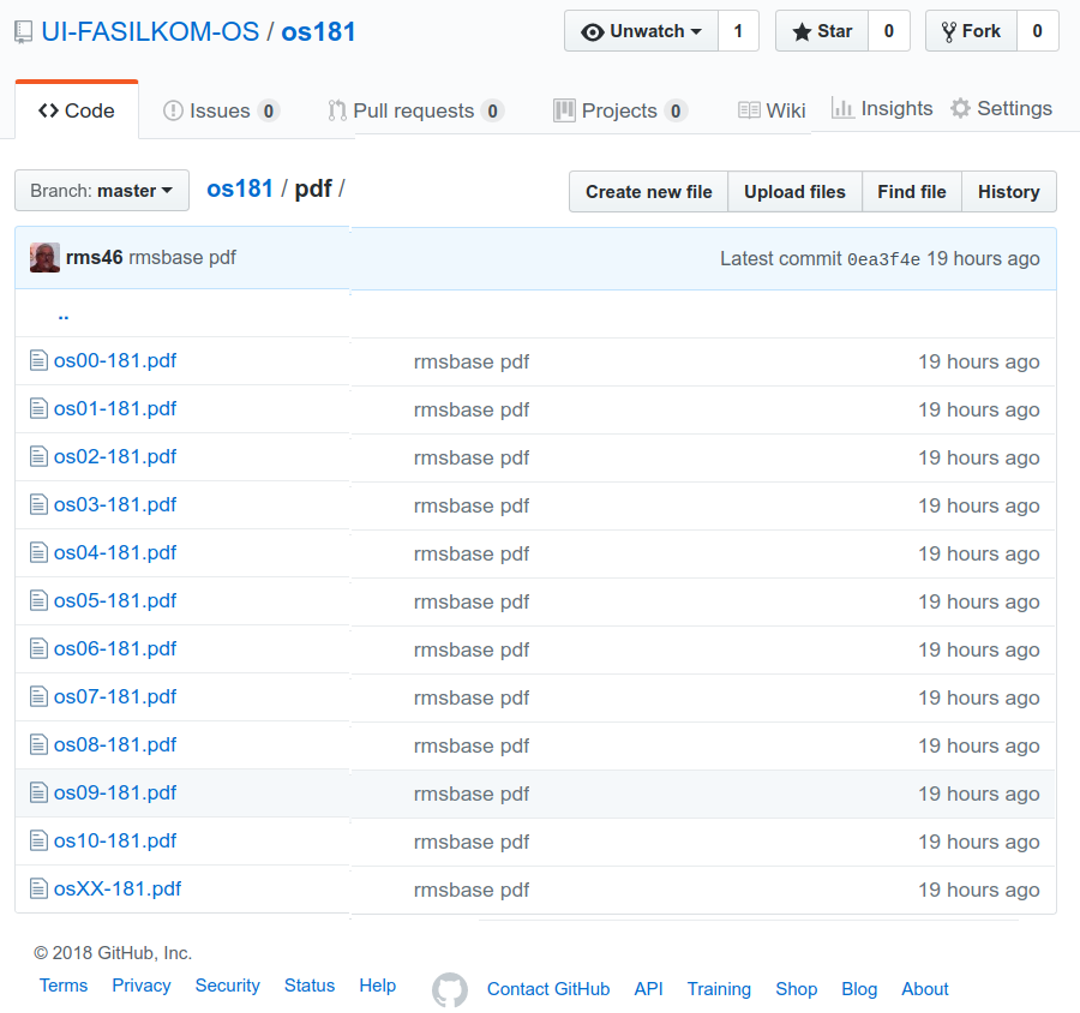
\includegraphics[width=0.55\linewidth]{os00-GIT}
\caption{\texttt{https://github.com/UI-FASILKOM-OS/os182/tree/master/pdf}}
\end{figure}
\end{frame}

% XXXXXXXXXXXXXXXXXXXXXXXXXXXXXXXXXXXXXXXXXXXXXXXXXXXXXXXXXXXXXXXXXXXXXXXXXX
\begin{frame}
\frametitle{Bahan Demo}
\begin{figure}
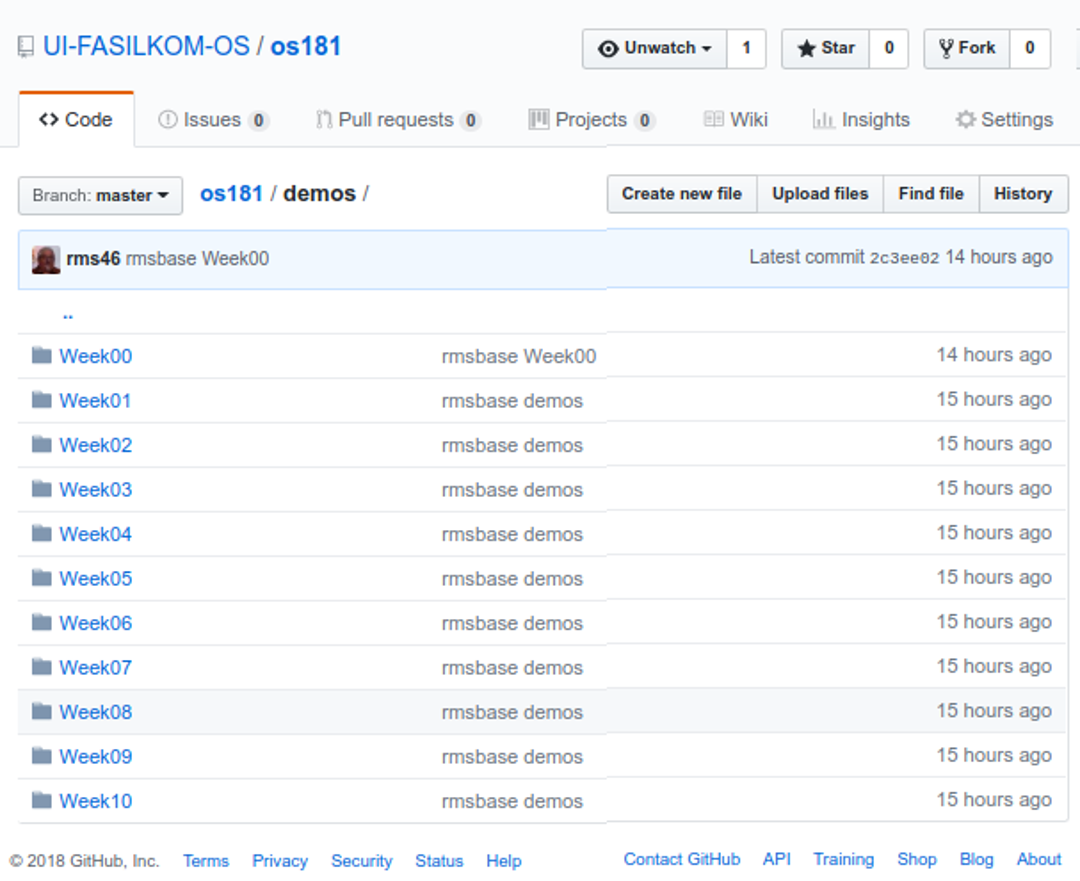
\includegraphics[width=0.73\linewidth]{os00-github-demo}
\caption{\texttt{https://github.com/UI-FASILKOM-OS/os182/tree/master/demos}}
\end{figure}
\end{frame}


% XXXXXXXXXXXXXXXXXXXXXXXXXXXXXXXXXXXXXXXXXXXXXXXXXXXXXXXXXXXXXXXXXXXXXXXXXX
\begin{frame}
\frametitle{Arsip SCELE}
\begin{figure}
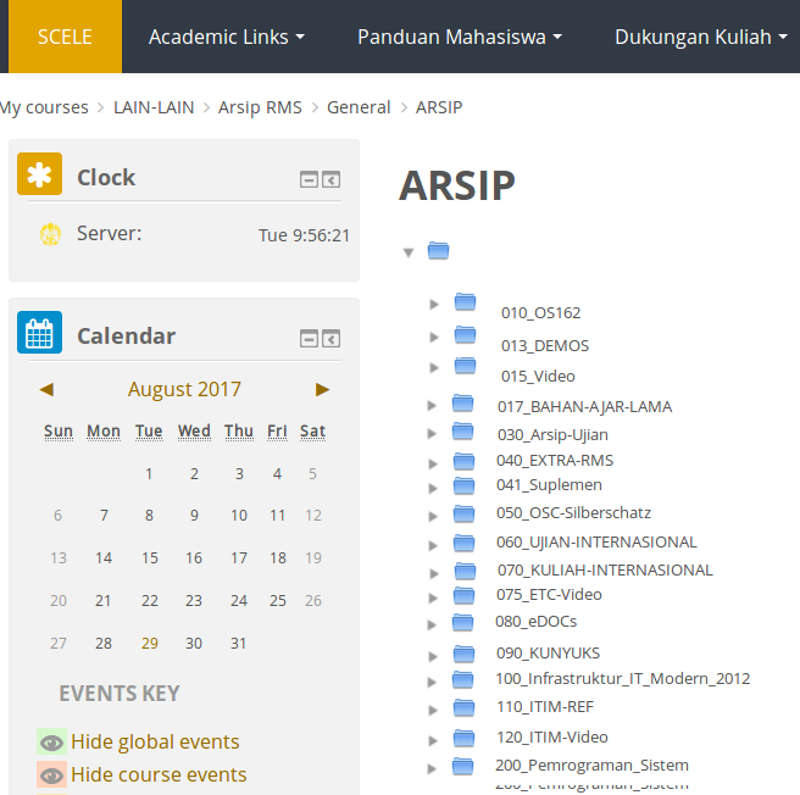
\includegraphics[width=0.60\linewidth]{os00-arsip-scele}
\caption{Lihat juga BADAK.cs.ui.ac.id:///extra/}
\end{figure}
\end{frame}

% XXXXXXXXXXXXXXXXXXXXXXXXXXXXXXXXXXXXXXXXXXXXXXXXXXXXXXXXXXXXXXXXXXXXXXXXXX
\section{Accounts}
\begin{frame}
\frametitle{Github (New) Account 1}
\begin{figure}
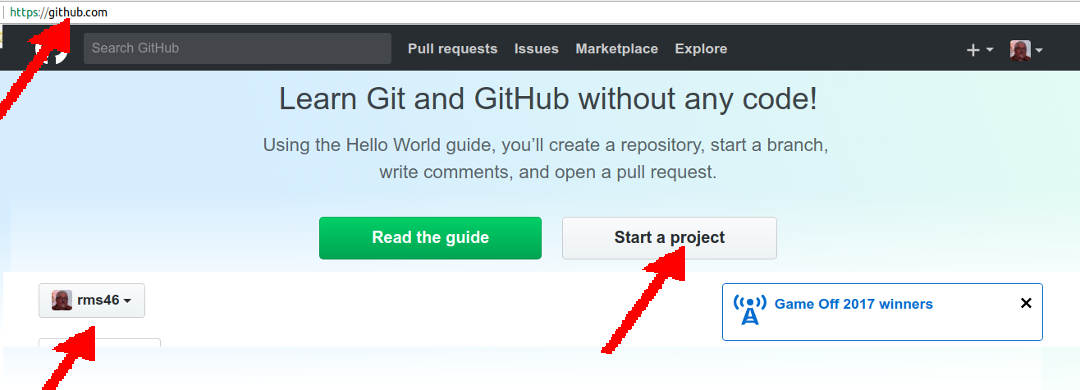
\includegraphics[width=0.91\linewidth]{os00-akun-git-1}
\caption{Start a new project by ''rms46''.}
\end{figure}
\end{frame}

% XXXXXXXXXXXXXXXXXXXXXXXXXXXXXXXXXXXXXXXXXXXXXXXXXXXXXXXXXXXXXXXXXXXXXXXXXX
\begin{frame}
\frametitle{Github (New) Account 2}
\begin{figure}
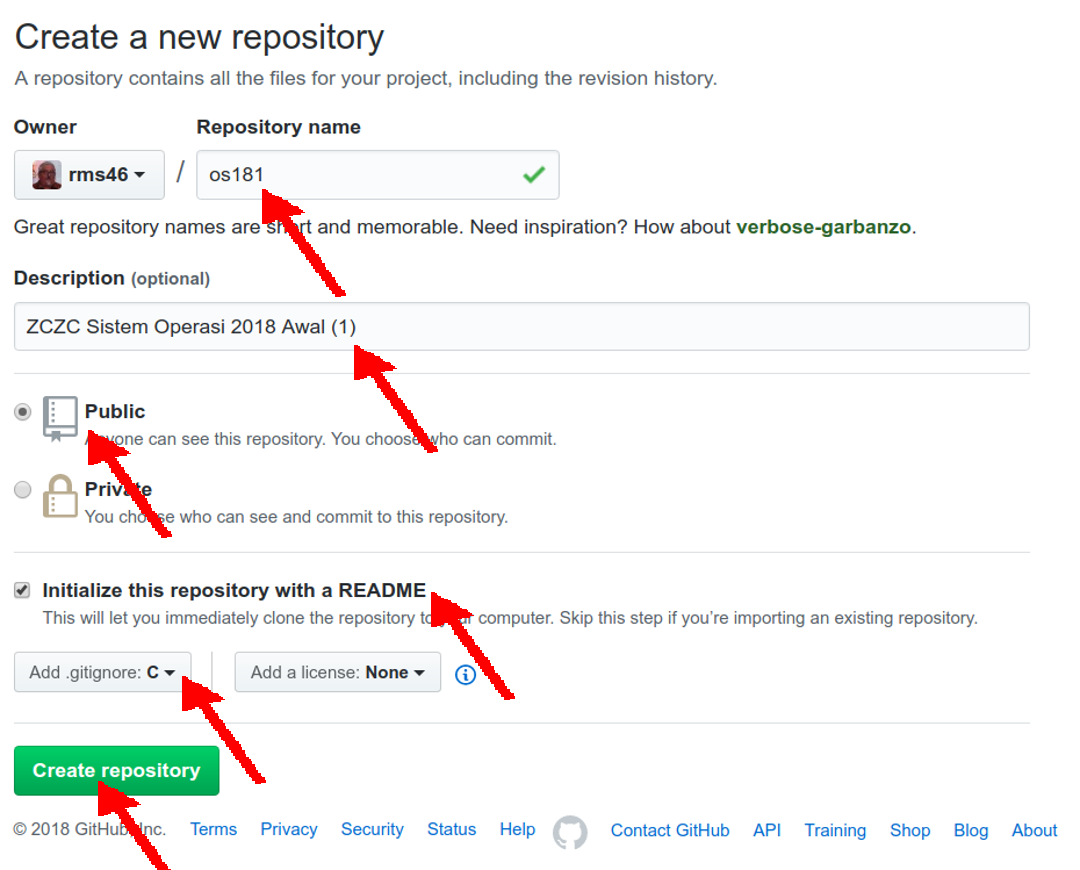
\includegraphics[width=0.70\linewidth]{os00-akun-git-2}
\caption{Create public repository ''os182'' with a README.md file}
\end{figure}
\end{frame}

% XXXXXXXXXXXXXXXXXXXXXXXXXXXXXXXXXXXXXXXXXXXXXXXXXXXXXXXXXXXXXXXXXXXXXXXXXX
\begin{frame}
\frametitle{Github (New) Account 3}
\begin{figure}
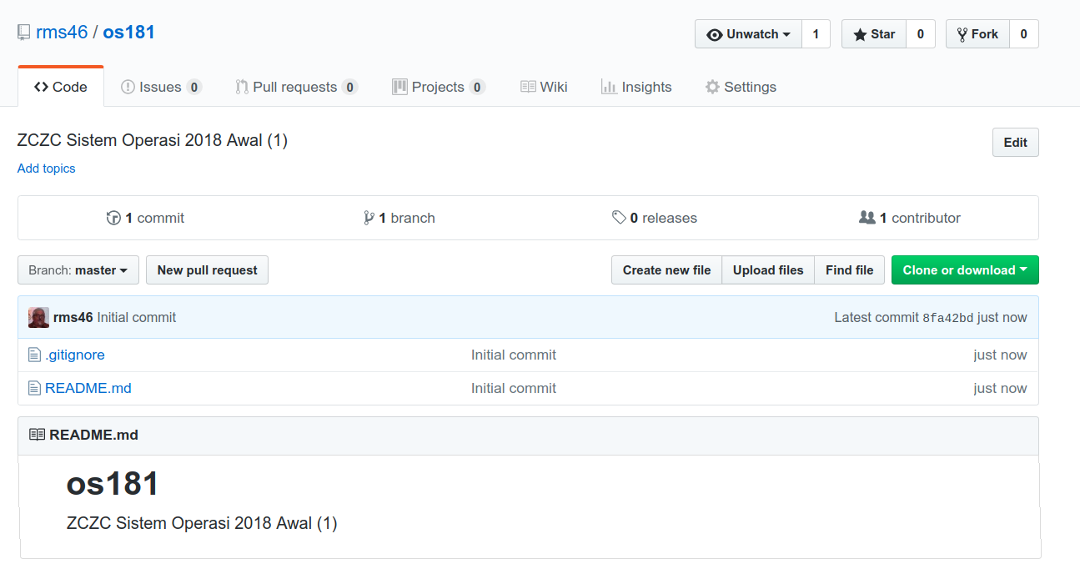
\includegraphics[width=0.91\linewidth]{os00-akun-git-3}
\caption{Public project ''os182'' by ''rms46'' at https://github.com/rms46/os182}
\end{figure}
\end{frame}

% XXXXXXXXXXXXXXXXXXXXXXXXXXXXXXXXXXXXXXXXXXXXXXXXXXXXXXXXXXXXXXXXXXXXXXXXXX
\begin{frame}
\frametitle{WSL: Windows Subsystem for Linux}
\begin{figure}
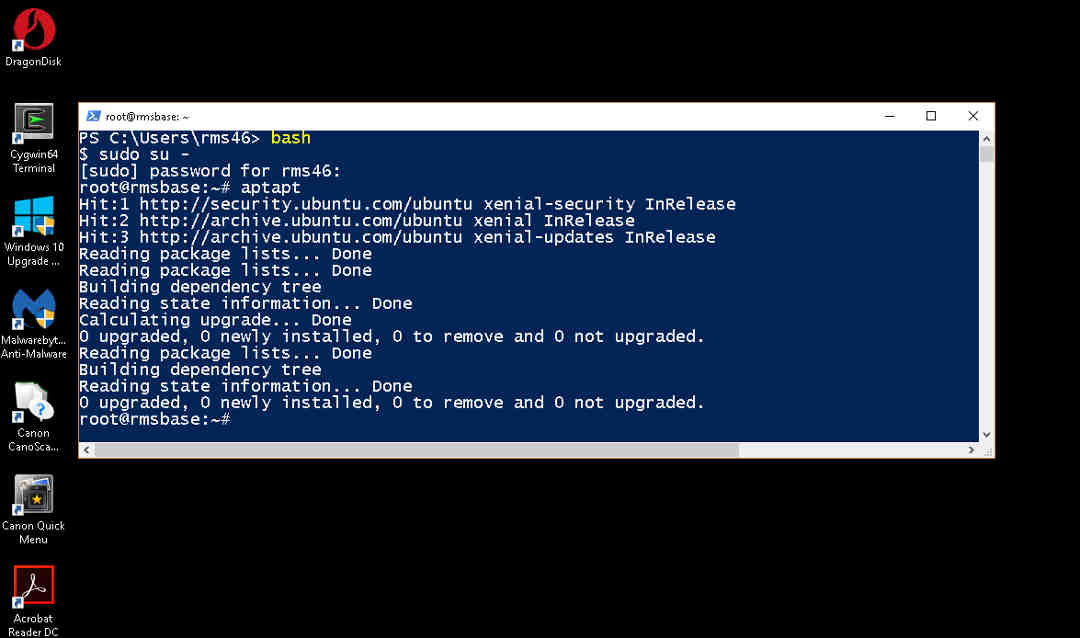
\includegraphics[width=0.95\linewidth]{os00-wsl-ubuntu-00}
\caption{WSL: Windows Subsystem for Linux}
\end{figure}
\end{frame}

% XXXXXXXXXXXXXXXXXXXXXXXXXXXXXXXXXXXXXXXXXXXXXXXXXXXXXXXXXXXXXXXXXXXXXXXXXX
\begin{frame}
\frametitle{Cygwin}
\begin{figure}
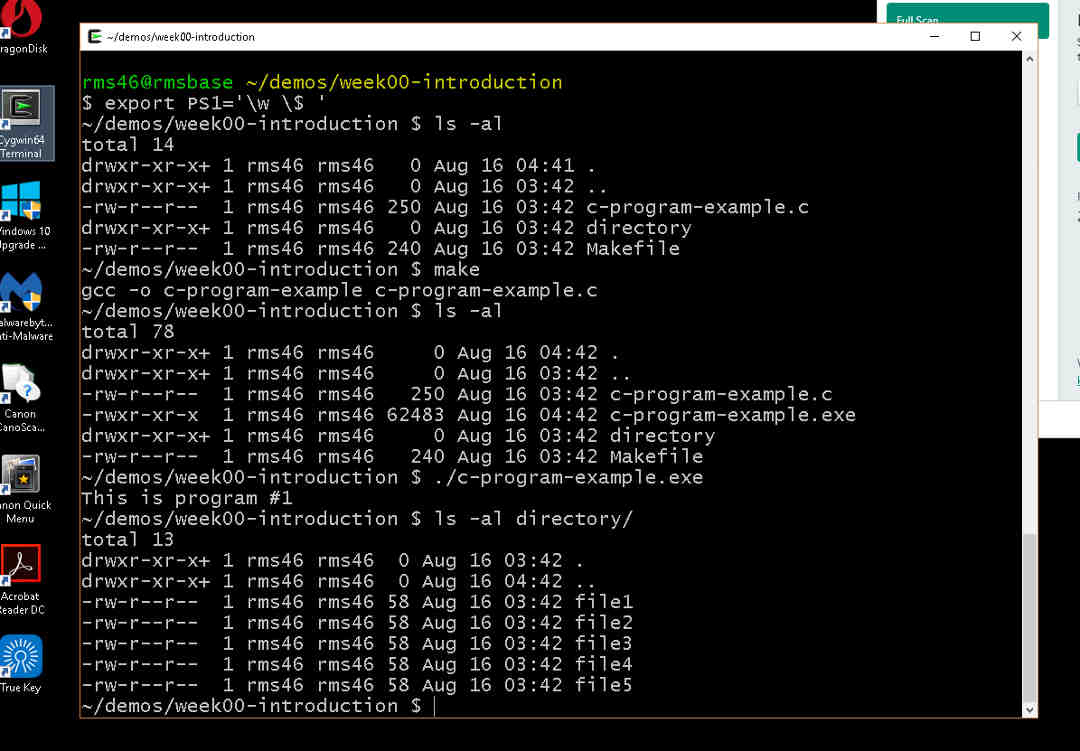
\includegraphics[width=0.85\linewidth]{os00-cygwin-01}
\caption{Cygwin}
\end{figure}
\end{frame}

% XXXXXXXXXXXXXXXXXXXXXXXXXXXXXXXXXXXXXXXXXXXXXXXXXXXXXXXXXXXXXXXXXXXXXXXXXX
\section{Week 00: Problems}
\begin{frame}
\frametitle{Week 00: Problems}
\begin{itemize}
\item Tugas Minggu 00 (Week 00) ada dua:
\begin{itemize}
\item membuat QRC dan mengirimkannya via email.
\item membuat Memo Minggu 00 yang ada QRC, serta ditunjukkan pada saat istirahat kuliah hari ke dua.
\end{itemize}
\item ''TANDA PETIK'' BUKAN merupakan bagian dari QRC!
\item Jangan mencantumkan ''.git'' dan ''.sso'', jika bukan bagian dari nama akun anda!
\item Tanpa header [W00] pada Subject; email anda mungkin akan nyasar entah kemana...
      Ingat: [W00] (We-Nol-Nol) tidak sama dengan [WOO] (We-O-O)!
\item Ukuran QRC cukup sekitar 256 x 256 pixel: jangan terlalu besar atau terlalu kecil.
\item QRC ditanam (embedded) dalam email; jangan menggunakan attachment!
\item Jangan mengirim MEMO dalam format PDF!
\end{itemize}
\end{frame}

% XXXXXXXXXXXXXXXXXXXXXXXXXXXXXXXXXXXXXXXXXXXXXXXXXXXXXXXXXXXXXXXXXXXXXXXXXX
\section{Week 00: Check List}
\begin{frame}
\frametitle{Week 00: Check List}
\begin{itemize}
\item[$\square$] Starting \textbf{Week 01}: TABULA RASA is not accepted anymore!
\item[$\square$] Find/copy this document from \texttt{http://os.vlsm.org/}
\item[$\square$] Find/read a recent/decent OS Book and map it to \textbf{OSC10}.
\item[$\square$] Using your \textbf{SSO} account, login to \texttt{badak.cs.ui.ac.id} via \texttt{kawung.cs.ui.ac.id}.
\item[$\square$] Check folder \texttt{badak:///extra/Week00/}
\begin{itemize}
\item[$\square$] Try to copy and compile \texttt{c-program-example.c}.
\end{itemize}
\item[$\square$] QR Code: (Eg) ''\texttt{OS182 X 1253755125 demo Demo Suremo}''
\item[$\square$] Mailto: \texttt{operatingsystems@vlsm.org} \\
                 (Eg.) Subject:  \texttt{OS182 X 1253755125 demo Demo Suremo}
\item[$\square$] Write ''Memo Week00'' + your QRC.
\item[$\square$] \textbf{How to improve this document?}
\end{itemize}
\end{frame}

% 12 XXXXXXXXXXXXXXXXXXXXXXXXXXXXXXXXXXXXXXXXXXXXXXXXXXXXXXXXXXXXXXXXXXXXXXX
% XXXXXXXXXXXXXXXXXXXXXXXXXXXXXXXXXXXXXXXXXXXXXXXXXXXXXXXXXXXXXXXXXXXXXXXXXX
\section{The End}
\begin{frame}
\frametitle{The End}
\begin{itemize}
\item[$\square$] This is the end of the presentation.
\item[$\boxtimes$] This is the end of the presentation.
\item This is the end of the presentation.
\end{itemize}
\end{frame}






% XXXXXXXXXXXXXXXXXXXXXXXXXXXXXXXXXXXXXXXXXXXXXXXXXXXXXXXXXXXXXXXXXXXXXXXXXX
\section{Week 00: Self Service Assignments}
\begin{frame}[fragile]
\frametitle{Week 00: Self Service Assignments}
\begin{itemize}
\item Create project (\textbf{PUBLIC}) "os182" on your new (or existing) github.com account.
\item (Week 00) QRCode\footnote{%
''QR Code'' is a registered trademark and wordmark of Denso Wave Inc.}: 
''OS182\\CLASS ID GITHUB-ACCOUNT SSO-ACCOUNT SIAK-Full-Name''
\item (Weekly)  Memo.
\item Informasi Kuliah, Arsip Ujian, dan Demo
\begin{itemize}
\item \texttt{badak.cs.ui.ac.id:/extra/}
\item \texttt{https://github.com/UI-FASILKOM-OS/os182}
\item \texttt{https://rms46.vlsm.org/2/195.pdf} --- [195.pdf - 205.pdf].
\end{itemize}
\item Which BASH Account?
\begin{itemize}
\item Virtual Ubuntu: badak.cs.ui.ac.id (SSO)
\item Ubuntu (BYOD)
\item WSL: Windows 10 Subsystem for Linux
\item Cygwin (Windows)
\end{itemize}
\end{itemize}
\end{frame}


% XXXXXXXXXXXXXXXXXXXXXXXXXXXXXXXXXXXXXXXXXXXXXXXXXXXXXXXXXXXXXXXXXXXXXXXXXX
\section{Week 01: Problems}
\begin{frame}
\frametitle{Week 01: Problems}
\begin{itemize}
\item Tugas Minggu 01 (Week 01) ada dua:
\begin{itemize}
\item Memo Week01: to be checked  at break of the first lecture of WEEK 01.
\item Try Demo Week01 and write in ''README.md'' (os181), something like:
                 ''ZCZC W01 Telah mencoba demo Week01''.
\end{itemize}
\end{itemize}

\begin{figure}
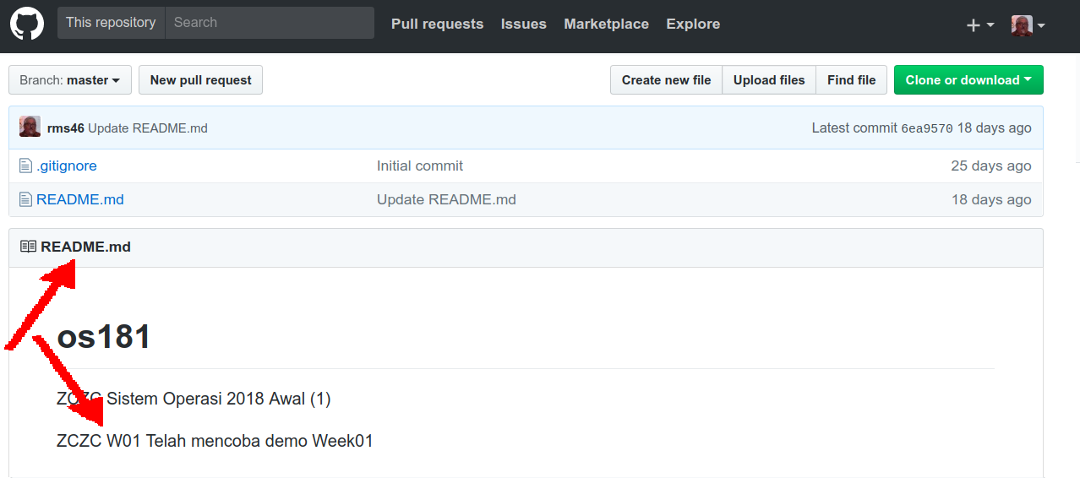
\includegraphics[width=0.85\linewidth]{os01-README}
\caption{README.md: ZCZC W01 \dots}
\end{figure}

\end{frame}


% XXXXXXXXXXXXXXXXXXXXXXXXXXXXXXXXXXXXXXXXXXXXXXXXXXXXXXXXXXXXXXXXXXXXXXXXXX
\section{Week 02: Problems}
\begin{frame}
\frametitle{Week 02: Problems}
\begin{itemize}
\item Tugas Minggu 02 (Week 02) ada dua:
\begin{itemize}
\item Memo Week02: to be checked  at break of the first lecture of WEEK 01.
\item Try Demo Week02 and write in ''README.md'' (os181), something like:
                 ''ZCZC W02 Demo: done!''.
\end{itemize}
\end{itemize}

\begin{figure}
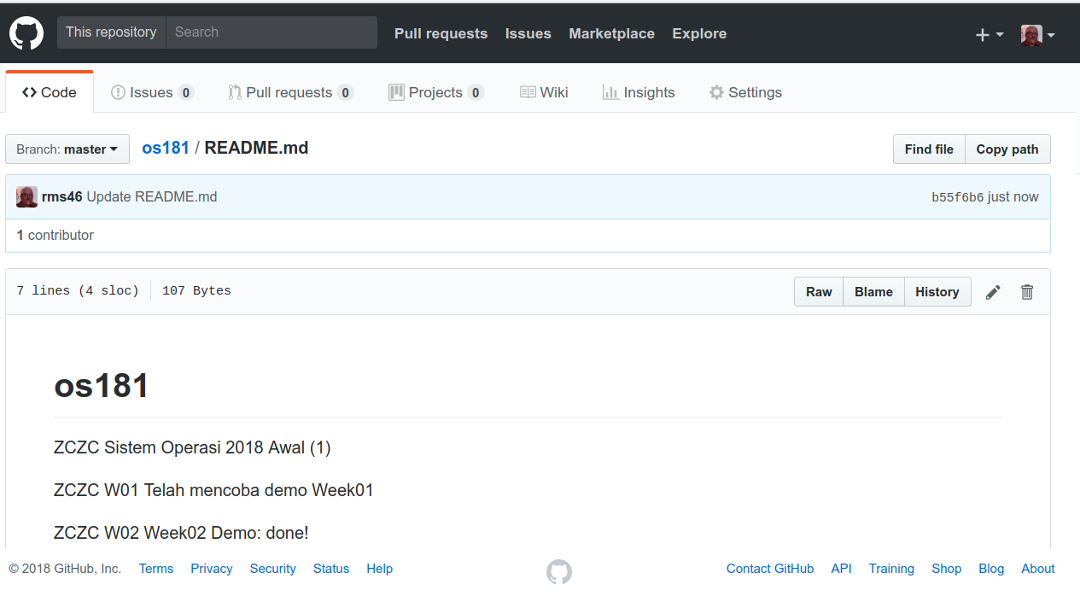
\includegraphics[width=0.80\linewidth]{os02-README}
\caption{README.md: ZCZC W02 Demo: done!}
\end{figure}

\end{frame}

% XXXXXXXXXXXXXXXXXXXXXXXXXXXXXXXXXXXXXXXXXXXXXXXXXXXXXXXXXXXXXXXXXXXXXXXXXX
\section{07-fork}
\begin{frame}[fragile]
\frametitle{07-fork}
% \begin{lstlisting}[basicstyle=\ttfamily\tiny]         % 108
% \begin{lstlisting}[basicstyle=\ttfamily\footnotesize] %  72
% \begin{lstlisting}[basicstyle=\ttfamily\small]        %  65
% \begin{lstlisting}[basicstyle=\ttfamily\large]        %  54
\begin{lstlisting}[basicstyle=\ttfamily\tiny]
>>>>> $ cat 07-fork.c 
/*
 * (c) 2005-2017 Rahmat M. Samik-Ibrahim
 * https://rahmatm.samik-ibrahim.vlsm.org/
 * This is free software.
 * REV05 Mon Oct 30 10:57:02 WIB 2017
 * REV02 Mon Oct 24 10:43:00 WIB 2016
 * REV01 Sun Feb 27 08:31:46 WIB 2011
 * START 2005
 */

#include <sys/types.h>
#include <sys/wait.h>
#include <stdio.h>
#include <stdlib.h>
#include <unistd.h>
#define DISPLAY1 "START * PARENT *** ** PID (%4d) ** **********\n"
#define DISPLAY2 "RANDOM: val1(%4d) -- val2(%4d) -- val3(%4d)\n"
/*************************************************** main ** */
void main(void) {
   pid_t val1, val2, val3;
   printf(DISPLAY1, getpid());
   val1 = fork();
   val2 = fork();
   val3 = fork();
   printf(DISPLAY2, val1, val2, val3);
   wait(NULL);
   wait(NULL);
   wait(NULL);
/* *********** START BLOCK ***
   *********** END * BLOCK *** */
}

\end{lstlisting}
\end{frame}

% XXXXXXXXXXXXXXXXXXXXXXXXXXXXXXXXXXXXXXXXXXXXXXXXXXXXXXXXXXXXXXXXXXXXXXXXXX
\begin{frame}[fragile]
\frametitle{07-fork (2)}
% \begin{lstlisting}[basicstyle=\ttfamily\tiny]         % 108
% \begin{lstlisting}[basicstyle=\ttfamily\footnotesize] %  72
% \begin{lstlisting}[basicstyle=\ttfamily\small]        %  65
% \begin{lstlisting}[basicstyle=\ttfamily\large]        %  54
\begin{lstlisting}[basicstyle=\ttfamily\tiny]

>>>>> $ 07-fork 
START * PARENT *** ** PID (6160) ** **********
RANDOM: val1(6161) -- val2(6162) -- val3(6163)
RANDOM: val1(6161) -- val2(6162) -- val3(   0)
RANDOM: val1(6161) -- val2(   0) -- val3(6165)
RANDOM: val1(6161) -- val2(   0) -- val3(   0)
RANDOM: val1(   0) -- val2(6164) -- val3(6166)
RANDOM: val1(   0) -- val2(6164) -- val3(   0)
RANDOM: val1(   0) -- val2(   0) -- val3(6167)
RANDOM: val1(   0) -- val2(   0) -- val3(   0)
>>>>> $ 07-fork 
START * PARENT *** ** PID (6168) ** **********
RANDOM: val1(6169) -- val2(6170) -- val3(6172)
RANDOM: val1(6169) -- val2(   0) -- val3(6173)
RANDOM: val1(6169) -- val2(6170) -- val3(   0)
RANDOM: val1(   0) -- val2(6171) -- val3(6174)
RANDOM: val1(6169) -- val2(   0) -- val3(   0)
RANDOM: val1(   0) -- val2(   0) -- val3(6175)
RANDOM: val1(   0) -- val2(   0) -- val3(   0)
RANDOM: val1(   0) -- val2(6171) -- val3(   0)
>>>>> $ 07-fork 
START * PARENT *** ** PID (6176) ** **********
RANDOM: val1(6177) -- val2(6178) -- val3(6181)
RANDOM: val1(   0) -- val2(6179) -- val3(6180)
RANDOM: val1(   0) -- val2(6179) -- val3(   0)
RANDOM: val1(   0) -- val2(   0) -- val3(6182)
RANDOM: val1(6177) -- val2(   0) -- val3(6183)
RANDOM: val1(6177) -- val2(   0) -- val3(   0)
RANDOM: val1(6177) -- val2(6178) -- val3(   0)
RANDOM: val1(   0) -- val2(   0) -- val3(   0)
>>>>> $ 
>>>>> $ 07-fork 

\end{lstlisting}
\end{frame}

% XXXXXXXXXXXXXXXXXXXXXXXXXXXXXXXXXXXXXXXXXXXXXXXXXXXXXXXXXXXXXXXXXXXXXXXXXX

% XXXXXXXXXXXXXXXXXXXXXXXXXXXXXXXXXXXXXXXXXXXXXXXXXXXXXXXXXXXXXXXXXXXXXXXXXX
\begin{frame}[fragile]
\frametitle{XXX}

\begin{itemize}
\item \textbf{4 SKS} (Units) means 12 hours per week!
\begin{itemize}
\item Ah Beng said: Work hard!
\end{itemize}
\item \textbf{No Lab --- No Task --- No Pop Quiz -- No Teaching Assistant}\footnotemark[\value{footnote}].
\begin{itemize}
\item No secret hand-shake!
\item But, it may vary from class to class.
\end{itemize}
\item \textbf{Active Preparation / Participation / Q\&A Only}.
\begin{itemize}
\item Pre-Midterm (UTS): 6 weeks @ 3 points (=18\%).
\item Post-Midterm: 5 weeks @ 3 points (=15\%).
\item Points for answering questions, trying demos, and writings memos.
\item Deductions for \textbf{NOT} answering questions: individually or collectively.
\end{itemize}
\end{itemize}

\end{frame}


% XXXXXXXXXXXXXXXXXXXXXXXXXXXXXXXXXXXXXXXXXXXXXXXXXXXXXXXXXXXXXXXXXXXXXXXXXX
\begin{frame}
\frametitle{Assessment part 2}

\begin{itemize}
\item \textbf{How to get points?}
\begin{itemize}
\item Answer questions, especially not in the middle of a lecture!
\item Try Demos.
\item Class attendance.
\end{itemize}
\item \textbf{MidTerm:} 6 set problems @ 6 points ( = 36\%).
\item \textbf{Final:} 30 points ( = 30\%)\footnote{THIS
       TERM ONLY. See
       \href{https://scele.cs.ui.ac.id/course/view.php?id=822}{SCELE}
       for more details!}.  \\
\item \textbf{Extra Rounding:} 1
%      point\footnote{Terms and Conditions apply. Void where prohibited by law.}  \\
       point\footnote{NOT AVAILABLE THIS TERM!}  \\
% \begin{itemize}
% \item Only if your grade is more than 59.0 and \textbf{ONE} more point.
% \end{itemize}
% \item \textbf{C-2C:} upto 5 points\footnotemark[\value{footnote}].
\item \textbf{C-2C:} upto 5 points \footnote{Terms
      and Conditions apply. Void where prohibited by law.}. \\
\begin{itemize}
\item Only if your grade is between 50.00 and 55.00 and you have a ''good'' track record.
\end{itemize}
\item Check your points regularly at \url{https://academic.ui.ac.id/} and
      \textbf{DO NOT COMPLAIN} weeks after! See also, \url{https://os.vlsm.org/}.
\end{itemize}

\end{frame}


% XXXXXXXXXXXXXXXXXXXXXXXXXXXXXXXXXXXXXXXXXXXXXXXXXXXXXXXXXXXXXXXXXXXXXXXXXXXXXXXXXXXXXXXXXXXXXXXXXXX
% 12 XXXXXXXXXXXXXXXXXXXXXXXXXXXXXXXXXXXXXXXXXXXXXXXXXXXXXXXXXXXXXXXXXXXXXXX
% XXXXXXXXXXXXXXXXXXXXXXXXXXXXXXXXXXXXXXXXXXXXXXXXXXXXXXXXXXXXXXXXXXXXXXXXXX
\section{The End}
\begin{frame}
\frametitle{The End}
\begin{itemize}
\item[$\square$] This is the end of the presentation.
\item[$\boxtimes$] This is the end of the presentation.
\item This is the end of the presentation.
\end{itemize}
\end{frame}

% XXXXXXXXXXXXXXXXXXXXXXXXXXXXXXXXXXXXXXXXXXXXXXXXXXXXXXXXXXXXXXXXXXXXXXXXXX
\end{document}

